\section{Results}
\label{sec:res}
Figure~\ref{fig:log_cm} shows the confusion matrix of the logistic regression model we discussed in Section~\ref{sec:log}. Among the 1000 testing data, 526 are spiral and 474 are elliptical. The accuracy of this model is 58.9\%, the precision is 55.8\% and the recall is 63.7\%. We can see that the accuracy is only slightly better than a random guess that should have the accuracy of 50\%. This lead us to believe that a more complex model is needed for this problem.

\begin{figure}[h]
	\centering
	\captionsetup{justification=centering}
	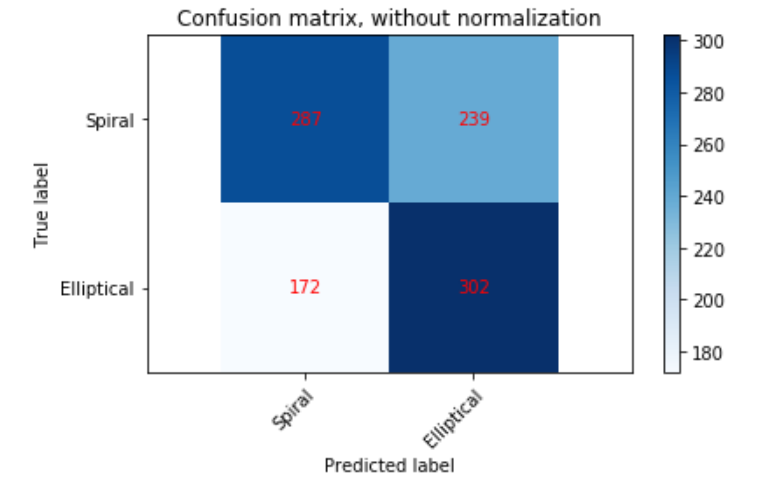
\includegraphics[width=0.6\columnwidth]{Figures/log_cm.png}
	\caption{Confusion matrix of testing data for the Logistic regression model}
	\label{fig:log_cm}
\end{figure}


\begin{figure}[h]
	\centering
	\captionsetup{justification=centering}
	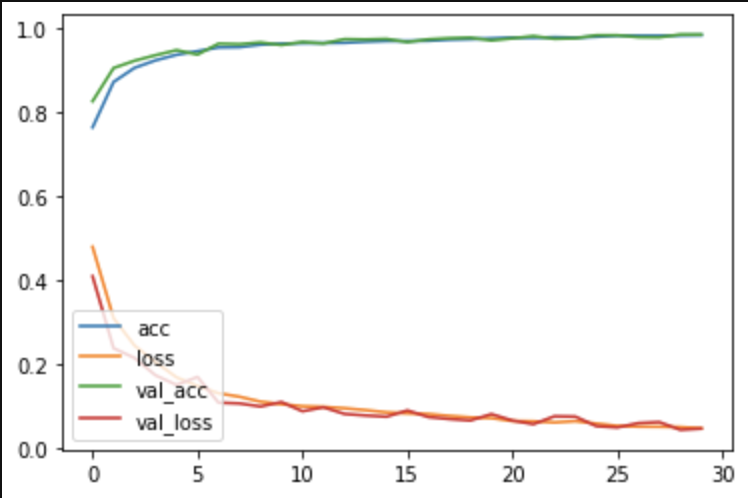
\includegraphics[width=0.4\columnwidth]{Figures/CNNMetrics.png}
	\caption{Training and validation metrics for the CNN model}
	\label{fig:cnnmetrics}
\end{figure}

Figure~\ref{fig:cnnmetrics} shows the plot of the training and validation results of CNN model we discussed in Section~\ref{sec:cnn}. 
We can see from the results that the CNN model is very promising, with a validation accuracy of 98.5\% over 30 epochs of training we can conclude that the a CNN is suitable for classifying the morphology of galaxies. With more training data and optimization of the model architecture and hypertuning the parameters the accuracy can be very well increased to over 99\%.